% ----------------------------------------
% Chap: Versuche auf dem EHD-Messgerät
% ----------------------------------------
\chapter{Versuche auf dem EHD-Messgerät}
\label{chap:versuche_auf_dem_ehd_messgeraet}

\improvement[inline]{Sagen, dass die Schmierfilmdickenmessung auch mit optisch ausgeführt wird.}

% ----------------------------------------
% Sec: Kapazitive Messgeräte zur Schmierfilmdickenbestimmung
% ----------------------------------------
\section{Kapazitive Messgeräte zur Schmierfilmdickenbestimmung}
\label{sec:kapazitive_messgeraete_zur_schmierfilmdickenbestimmung}

% ----------------------------------------
% Sub: Stromladekurve Messgerät
% ----------------------------------------
\subsection{Stromladekurve Messgerät}
\label{sub:stromladekurve_messgeraet}

Im IMKT gibt es ein mobiles Messsystem zur Schmierfilmdickenmessung mittels kapazitiven Messverfahren.
Das System besteht aus einem Laptop, der mit \textit{Laderkurve-Software} installiert, und einer Messkarte (Typ USB-6211) von der Firma National Instrument (NI).

Bei kapazitiver Messmethode wird der EHD-Kontakt als ein Kondensator ($C_K$) betrachtet.
Die Auflade des Kondensators erfolgt durch eine Ladespannung $U_L$ (\SIrange{0,2}{0,5}{\volt}) und einen Vorwiderstand $R_V$ (\SI{1012.7}{\kilo\ohm}).
Eine unendliche Erhöhung der Ladespannung ist aber unerwünscht, weil die zur Ionisierung des Schmierstoffes bei hohen Spannung verursacht und das kann die Messergebnisse verfälschen.
Abbildung \ref{fig:Schematischer_aufbau_des_mobilen_messsystems} zeigt das Prinzip des mobilen Messsystems zur Schmierfilmdickenmessung bei IMKT an.
% ----------------------------------------
% Fig: Schematischer Aufbau des mobilen Messsystems
% ----------------------------------------
\begin{figure}[htb]
    \centering
    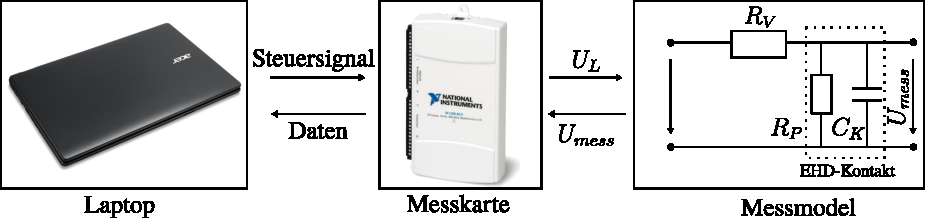
\includegraphics[]{./images/schematischer_aufbau_des_mobilen_messsystem.pdf}
    \caption{Schematischer Aufbau des mobilen Messsystems}
    \label{fig:Schematischer_aufbau_des_mobilen_messsystems}
\end{figure}

Das ganze Messsystem wird von der \textit{Laderkurve-Software} gesteuert.
Sie miss nicht direkt die Kapazität, sondern nimmt sie die Antwort bzw. Ladekurve des ``Kondensators'' auf, danach wird die Auswertung mit einem Matlab-Skript ausgeführt.
Die Software kann die Ladekurve in zwei Modi: \emph{Anzahl der Messwerte} oder \emph{Messung nach Zeit} aufnehmen.
Im Rahmen dieser Arbeit werden alle Messungen mit dem ersten Modus gemacht.
Abbildung \ref{fig:gui_der_laderkurve_software} zeigt die Benutzeroberfläche der Ladekurve-Software bei einer Testmessung mit einem Referenz-Kondensator (\SI{3.3}{\nano\farad}) an.
% ----------------------------------------
% Fig: GUI der Ladekurve-Software
% ----------------------------------------
\begin{figure}[htb]
    \centering
    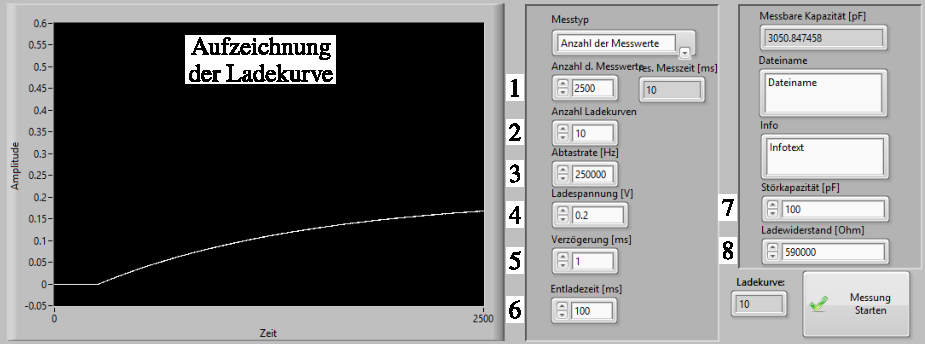
\includegraphics[]{./images/ladekurven_gui.pdf}
    \caption{Benutzeroberfläche der Laderkurve-Software}
    \label{fig:gui_der_laderkurve_software}
\end{figure}

Die Software ist relative einfach zu bedienen, allerdings gibt es folgende Punkte, auf die man beachten muss.
\begin{description}
    \item[1. Anzahl der Messwerte] ist die Auflösung der Messung.
        Zu niedriger Wert kann zum Messfehler führen und zu hohen Wert kann es schnell den Speicher voll machen, außerdem ist sie auch von der Abtastrate der Messkarte beschränkt.
        Der Standardwert ist \num{2500}.

    \item[2. Anzahl der Ladekurven] ist die Anzahl der Messungen, die nach einander durchgeführt werden. ist die Anzahl der Messungen, die nach einander durchgeführt werden.
        Der Standardwert ist \num{10}.

    \item[3. Abtastrate] ist die Anzahl der Messwerte, die Messkarte pro Sekunde messen kann.
        Die USB-6211 Messkarte von NI kann maximal \SI[per-mode=symbol]{250}{\kilo\sample\per\second}, das entspricht \num{2500} Messwerte in einem Zeitraum von \SI{10}{\milli\second}.

    \item[4. Ladespannung] ist die Spannung zwischen zwei Terminal des Kondensators.
        Der Wert sollte im Bereich von \SIrange{0.2}{0.5}{\volt} liegen.

    \item[5. Verzögerung] ist die Wartezeit, die die Software warten muss, bevor sie eine Messung ausführt.
        Der Standardwert ist \SI{1}{\ms}.

    \item[6. Entladezeit] ist die Zeit zwischen zwei Messungen.
        Sie ist notwendig, um der Kondensator komplette leer bevor jeder neuen Messung zu entladen.
        Der Standardwert ist \SI{100}{\ms}.

    \item[7. Ladewiderstand] ist der Wert des Vorwiderstands.
        Er ist nur für den Dokumentationszweck und wird in der Messdatei geschrieben.

    \item[8. Störkapazität] ist die externe Störung, wie zum Beispiel von Messkabel oder statische Kapazität zwischen Messkörpern.
        Dieser Wert wird für die spätere Auswertung verwendet.

    \item[9. Austecken des Netzteils] ist notwendig, um die Störungen von anderen elektronischen Geräte zu vermeiden.
\end{description}

%
% ----------------------------------------
% Sub: LCR Messgerät
% ----------------------------------------
\subsection{LCR Messgerät}
\label{sub:lcr_messgeraet}

In der Praxis kann jede Flüssigkeit und jeder Feststoff Strom durchlassen.
Wenn das Material von einem Wechselstrom gespeist wird, wird das Verhältnis zwischen der Spannung und dem Strom als Impedanz bezeichnet.
Die Veränderung der gemessenen Impedanz durch die Variation der Stromfrequenz ist von der Eigenschaft des Materials abhängig.
Das kann auf die physikalische Struktur des Werkstoffes, auf die innere chemische Prozesse oder eine Kombination von beiden zurückführen.
Der Zusammenhang zwischen der Impedanz, der Frequenz und der Kapazität von einem mit Wechselstrom angelegten Kondensators wird in der Formel \ref{eq:impedanz_kondensator} \cite{impedance} dargestellt.
%
\begin{equation}
    Z_{C} = \cfrac{v_C(t)}{i_C(t)} = \cfrac{1}{j \omega C}
    \label{eq:impedanz_kondensator}
\end{equation}

Im Gegenteil zum mobilen Ladekurve-Messsystem, welches die Kapazität über die Antwort einer Ladespannung interpretiert, bietet das LCR-Messgerät ST2826 der Firma Sourcetronic die Möglichkeit, die Kapazität eines EHD-Kontakts direkt zu messen.
Abbildung \ref{fig:versuchsaufbau_zur_kapazitaetsmessung_mit_lcr_meter} zeigt den Aufbau des Messsystems mit dem LCR-Messgerät.
% ----------------------------------------
% Fig: Schematischer Aufbau des Messsystems mit LCR-Meter
% ----------------------------------------
\begin{figure}[htb]
    \centering
    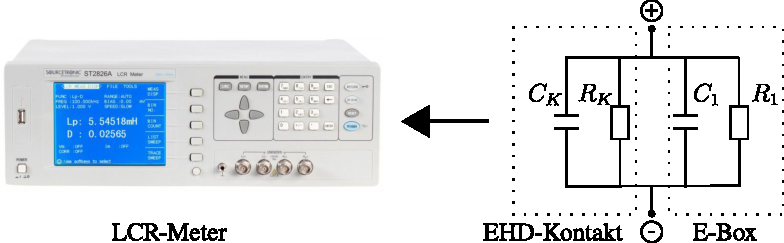
\includegraphics[]{./images/versuchsaufbau_mit_lcr_meter.pdf}
    \caption{Versuchsaufbau zur Kapazitätsmessung mit LCR-Meter}
    \label{fig:versuchsaufbau_zur_kapazitaetsmessung_mit_lcr_meter}
\end{figure}

Das LCR-Messgerät bietet einen breiten Frequenzbereich von \SI{20}{\Hz} bis \SI{50}{\MHz}.
Dank der Kelvin-Messproben (4-Punkt Messung) hat das Gerät eine sehr gute Genauigkeit von \SI{0.1}{\percent} und ermöglicht die Messung auch bei kleinsten Änderung des Systems.
Mit einer Sinuskorrelationstechnik bietet das Gerät eine rauschfreie Analyse.
Die Addition des Widerstands $R_1$ und des Kondensators $C_1$ sind benötigt, um zu sehen, ob der Strom tatsächlich durch den EHD-Kontakt fließt oder in irgeneiner Verbindung verloren geht.
Unterschiedliche Werte für $R_1$ und $C_1$ wurden verwendet, um deren Einfluß auf die gemessene Kapazität zu untersuchen.
Ein Erhöhung des Widerstandswertes führt zu einer signifikanten Abnahme der Messergebnisse und umgekehrt.
Dieses Phänomen kann durch die Abnahme bzw. Zunahme des Stromflusses durch den EHD-Kontakt erklärt werden.
Die Werte $R_1 = 2$ \si{\kilo\ohm} und $C_1 = 24$ \si{\pico\farad} wurden durch Experiment für weitere Messungen in dieser Arbeit gewählt.
Abbildung \ref{fig:lcr_ebox_capacitance} zeigt die Kapazitätsmessung des E-Box (offen) mit dem LCR-Messgerät bei verschiedenen Frequenzen.
% ----------------------------------------
% Fig: Messprobe mit 24 pF mit dem LCR-Meter
% ----------------------------------------
\begin{figure}[htb]
    \centering
    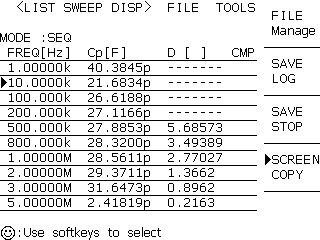
\includegraphics[width=0.5\linewidth]{./images/lcr_ebox_capacitance.jpg}
    \caption{Kapazitätsmessung des E-Box mit dem LCR-Messgerät}
    \label{fig:lcr_ebox_capacitance}
\end{figure}

% ----------------------------------------
% Sec: Versuchdurchführung
% ----------------------------------------
\section{Versuchdurchführung}
\label{sec:versuchdurchfuehrung}
\improvement[inline]{Schreiben der Versuchdurchführung}


Da die Auswertung der Schmierfilmdicke in dieser Arbeit optisch und elektrisch geschieht wird, ist die Sauberkeit vor dem Beginn einer Messung besonders wichtig zu achten.
Die Glasscheibe, die Kugel, das Kugelsupport und das Ölreservoir müssen vor jeder Messung mit Waschbenzin oder Isopropanol gereinigt werden und dürfen keine Schlieren aufweisen.

Nach der Reinigung können das Support und die Kugel in das Gerät eingesetzt werden.
Die Führung der Kugel wird zuerst in die Ausgangswelle des zweiten Motors eingesteckt und dann auf das Support aufgelegt.
Die Kabel sollen Abstand von den Wände des Reservoirs und der Motorwelle gehalten werden, um ein Unfall (Kurzschluss der Kugel, Verfangen des Kabels) während des Betriebs zu vermeiden.
Die Abbildung \ref{fig:ehd_topf_mit_kugel_und_support} zeigt den Blick von oben des EHD-Prüftopfs mit montierten Support und aufgelegter Kugel bereits für den Versuch.
% ----------------------------------------
% Fig: EHD-Prüftopf mit montierten Support und Modifizierter Kugelführung
% ----------------------------------------
\begin{figure}[htb]
    \centering
    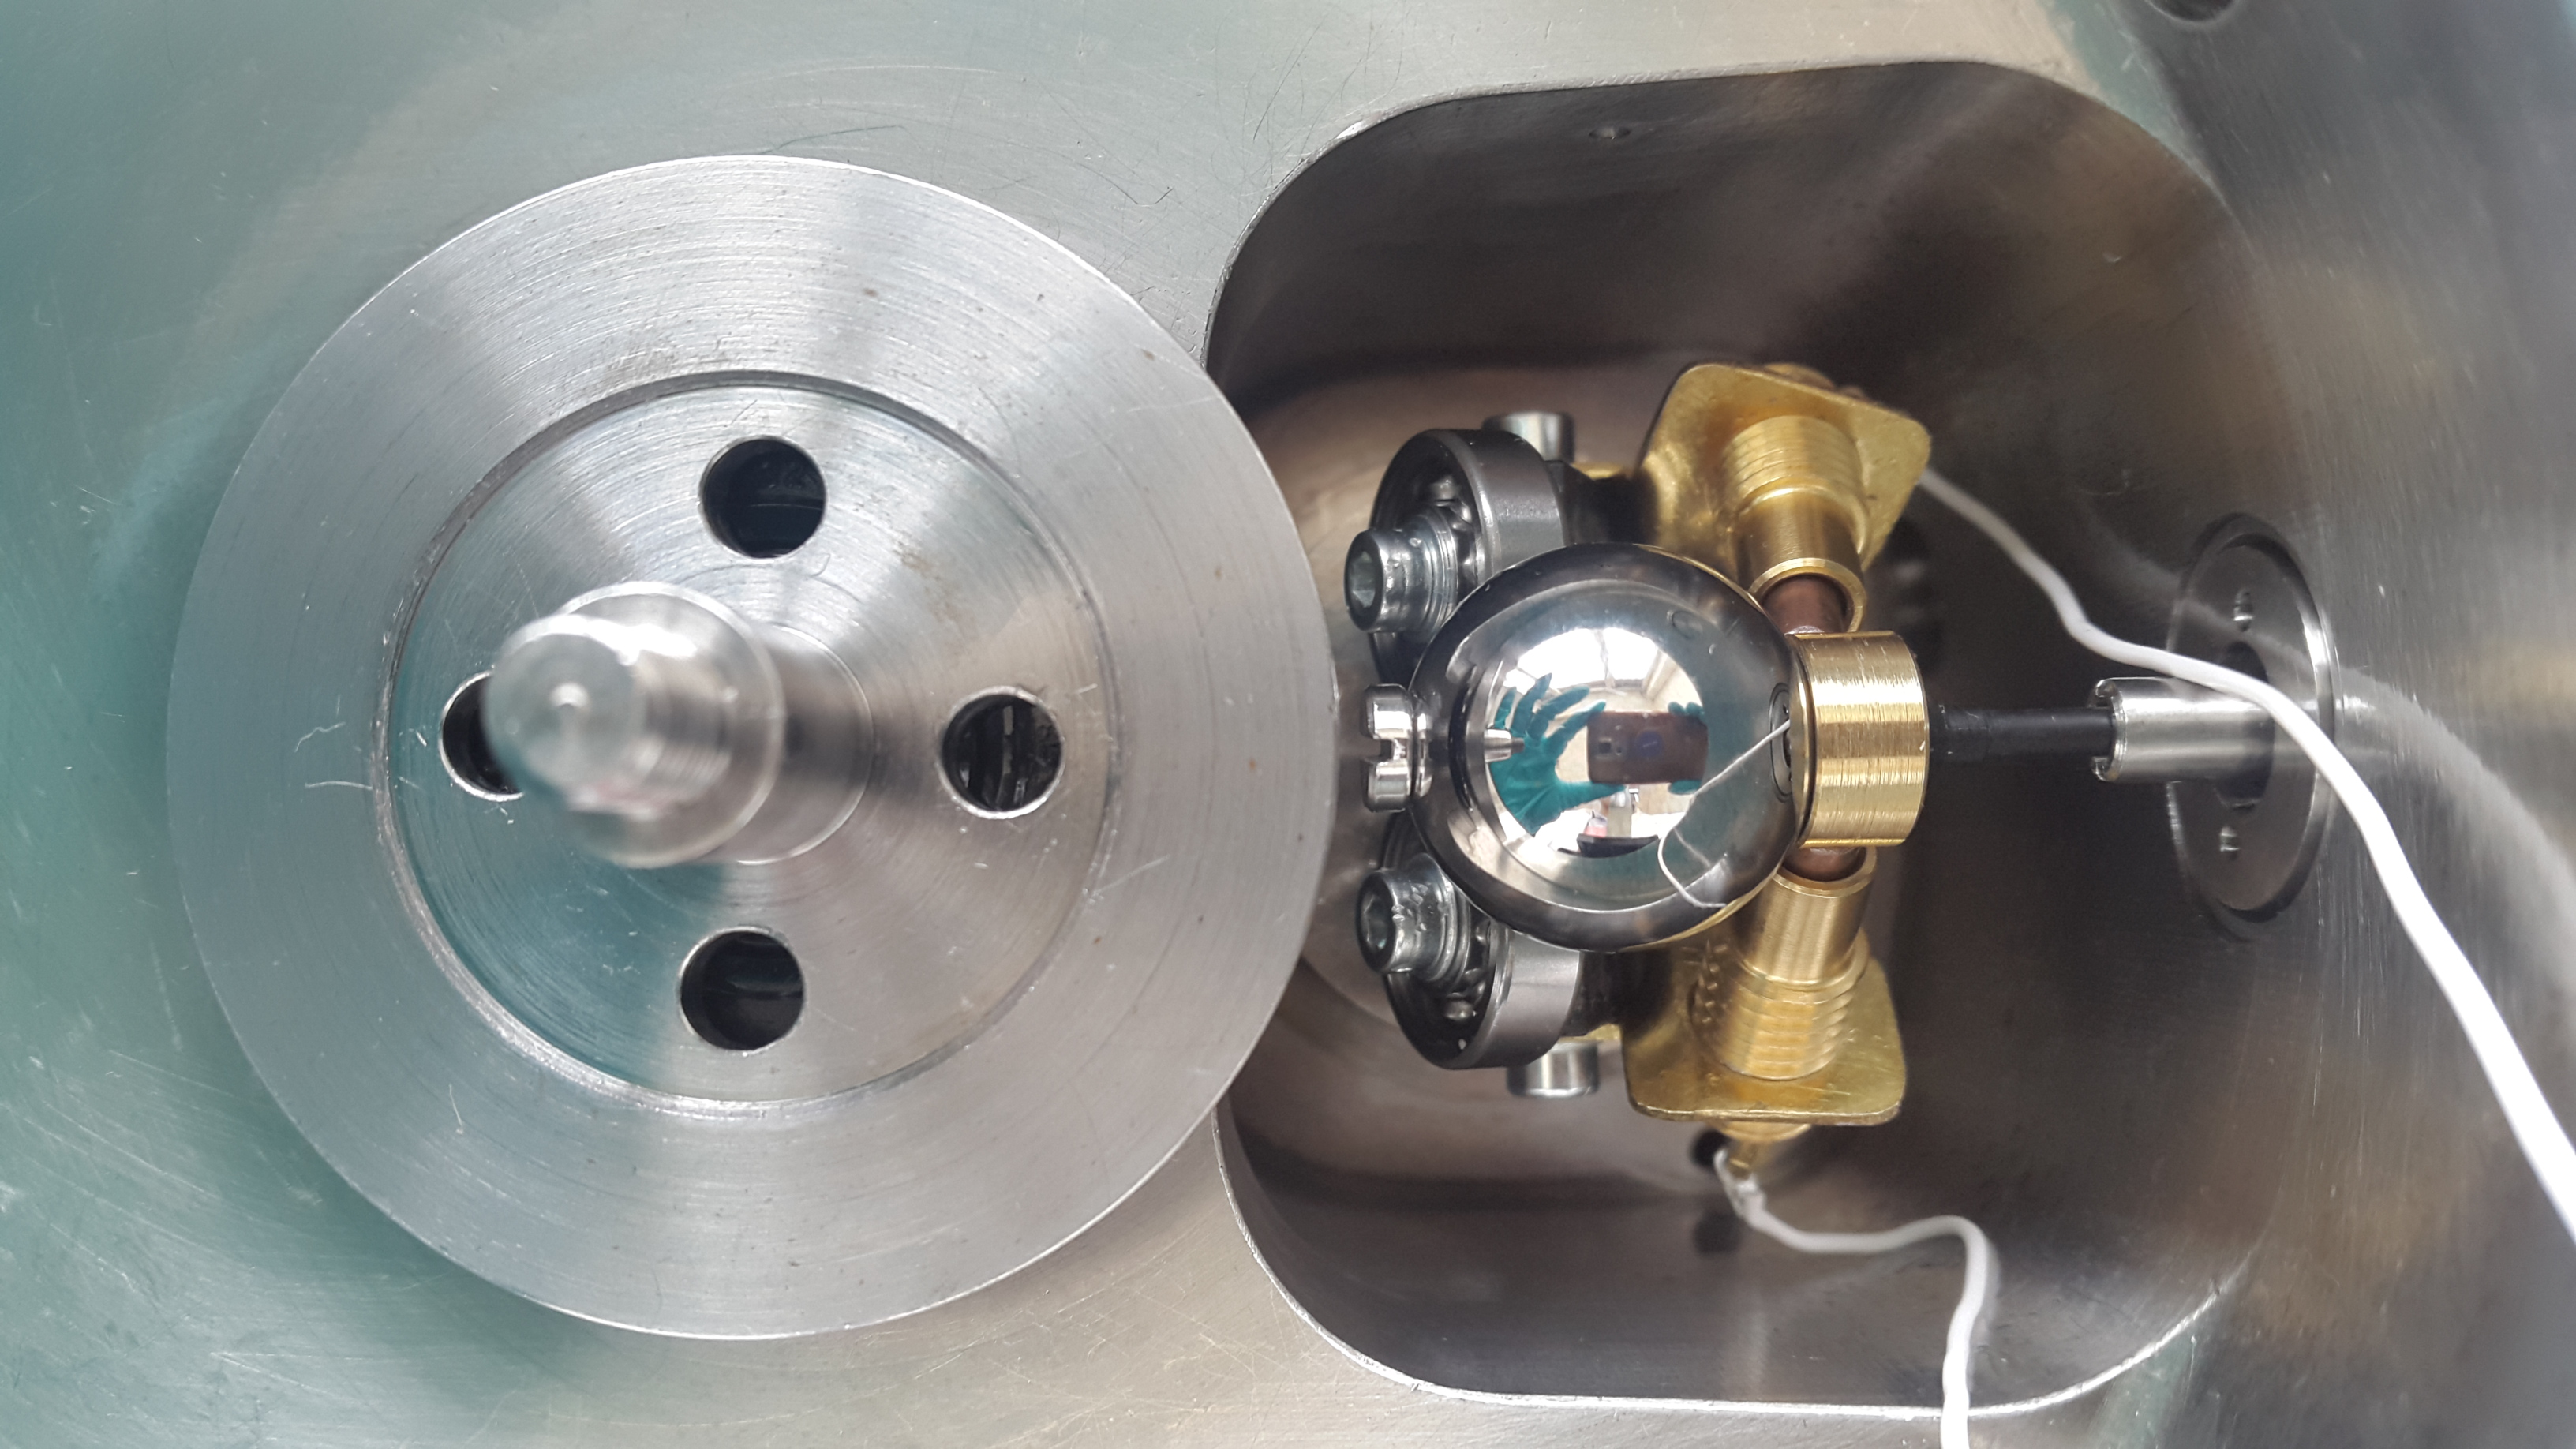
\includegraphics[width=0.8\linewidth]{./images/ehd_topf_mit_kugel_und_support.jpg}
    \caption{Topf des EHD-Geräts mit montierten neuen Kugelsupport und der Modifizierter Kugelführung}
    \label{fig:ehd_topf_mit_kugel_und_support}
\end{figure}

Die Bestimmung des Messpunkts für die optische Messung erfolgt zuerst auf der nicht beschichteten Seite der Scheibe.
Da nach wird die Scheibe \SI{180}{\degree} auf der Cr-Seite gedreht, um der Widerstand der gesamten Messkette (Kabel -> Scheibe -> Kugel -> Kabel) unter einer Last von \SI{20}{\newton} zu vermessen.
Er ist von dem Radius der Fahrspur abhängig und beträgt ungefähr \SIrange{17}{18}{\ohm}.
Die Suche nach dem Messpunkt passiert beim leeren Reservoir, weil ein sauberer Kontakt zwischen Scheibe und Kugel für die Bestimmung der Höhe des Spacer-Layers nötig ist.
Außerdem darf man nur das Spurwechseln beim leeren Zustand machen, weil das Verlaufen des Öles über die Lasteinheit in mechanischen Baukasten zum Schaden führen kann.
Man sollte die Spur von außen nach innen wechseln, um die Entstehung der Insel, die elektronisch zu den Elektroden (Kupferstreifen) isoliert sind, zu vermeiden.
Danach kann man das Öl mit der Hilfe einem Trichter befüllen und den Prüftopf mit dem Deckel zu machen.
Abbildung \ref{fig:ehd_kontakt} zeigt den gut auswertbaren und schlechten EHD-Kontakte an.
% ----------------------------------------
% Fig: Bestimmung des Messpunkts
% ----------------------------------------
\begin{figure}[htb]
    \centering
    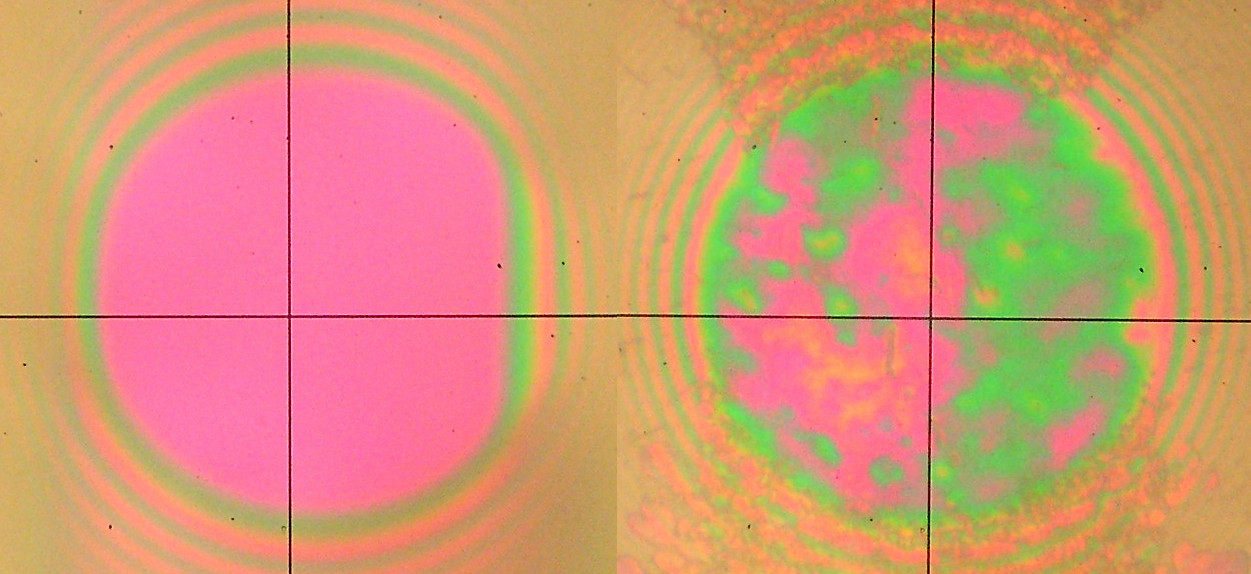
\includegraphics[width=0.8\linewidth]{./images/ehd_kontakt.jpg}
    \caption{EHD-Kontakt: gut auswertbarer Kontakt (rechts); schlechter Kontakt (links)}
    \label{fig:ehd_kontakt}
\end{figure}

Zur Messung bei Öl-Vollschmierung wird das Ölreservoir bis zur Hälfte der Kugel (ca. \SI{120}{\ml}) gefüllt.
Das Ölbad wird vor jeder Messreihe während des Heizvorgangs (bei \SI{40}{\degreeCelsius}, \SI{60}{\degreeCelsius} und \SI{80}{\degreeCelsius}) für ca. \SI{10}{\minute} durchmischt, um eine homogene Temperatur im Ölbad beim Versuch zu herrschen.
Das genaue Vorgehen einer solchen Messung wurde von \textit{Surborg} in seiner Arbeit \cite{surborg_2007} beschrieben und ist im Anhang zu finden.

Neben dem Widerstand des Kontakts wird die Hintergrund-Kapazität des Prüfstands auch gemessen.
Dieser Wert wird als Störkapazität bezeichnet und soll von der Ergebnissen beseitigt werden.

Die Last von \SI{20}{\newton} wird in Anlehnung an vorherigen Arbeiten gewählt.
Nach dem Abschnitt \ref{sec:betrachtung_des_ehd_kontaktes} lässt es sich für den hier betrachteten Fall eines Kugel-Scheibe-Modells eine maximale Pressung im Kontakt $p_0 =$ \SI{505}{\mega\pascal} berechnen.
Damit liegt der Kontakt im unteren Bereich der EHD-Schmierung.
Diese geringe Last ist gut, somit wird die Gefahr von Beschädigung auf der Scheibe bzw. der Silikatschicht gering gehalten.

Nachdem die Höhe des Spacer-Layers bestimmt wurde, wird die Scheibe ein Stück weiter gedreht und auf etwa \SI[per-mode=symbol]{100}{\mm\per\second} beschleunigt.
Während dieser Einlaufphase wird ständig das Live Bild auf dem SW-Monitor beobachtet.
Sobald sich ein klarer, gut messbarer Verlauf abzeichnet (siehe Abbildung \ref{fig:ehd_live_bild}), kann man mit der Messung begonnen werden.
Wichtig ist, dass man die Messungen zügig machen soll, um die Beschädigung der Chromschicht und Silikatschicht zu vermeiden.
% ----------------------------------------
% Fig: Schlechtes und gutes Live Bild
% ----------------------------------------
\begin{figure}[htb]
    \centering
    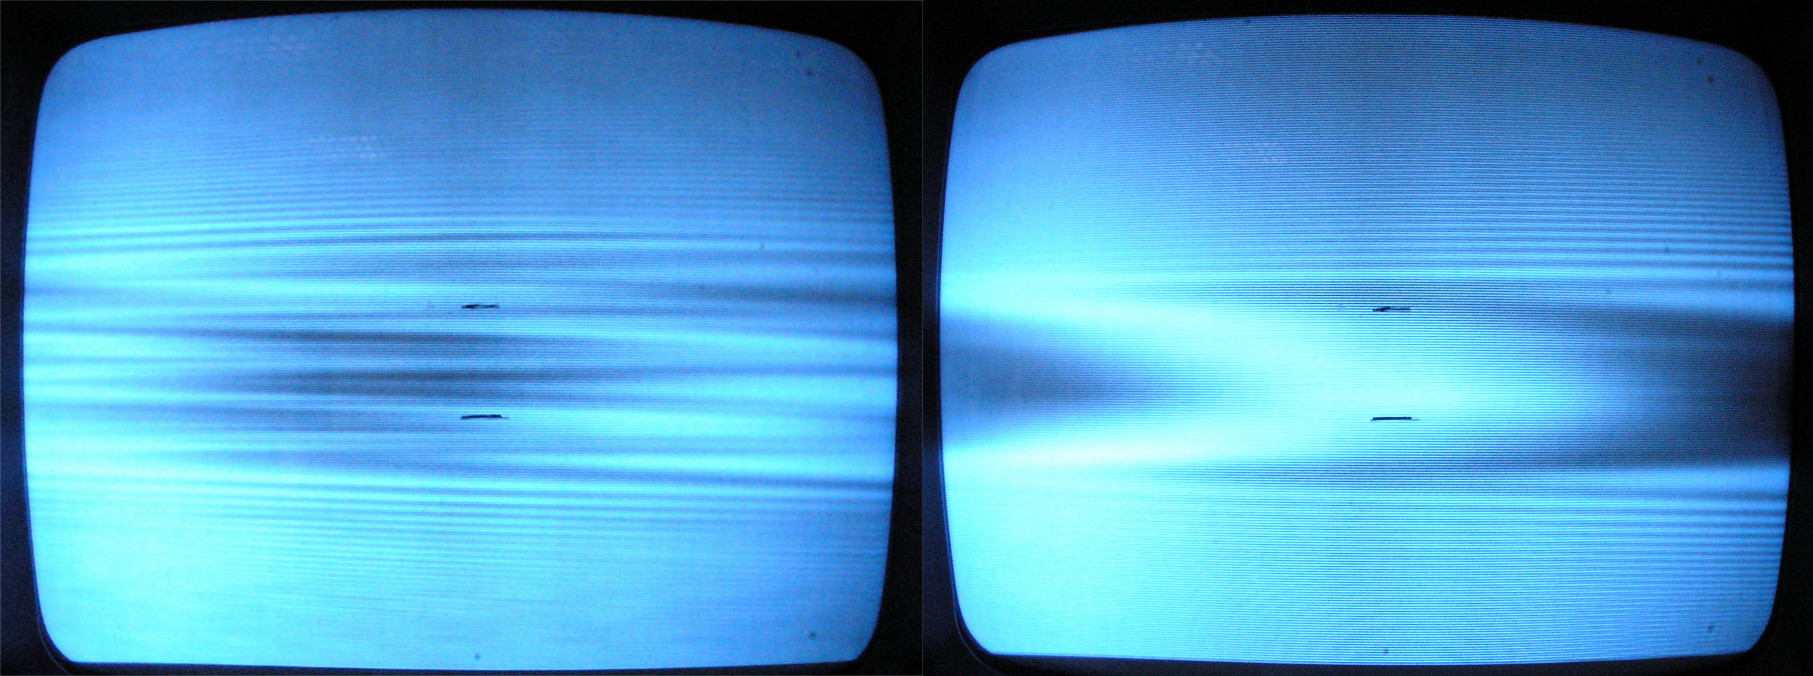
\includegraphics[width=0.8\linewidth]{./images/ehd_live_bild.jpg}
    \caption{Live Bild: nicht verwertbarer Verlauf (links); guter Verlauf (rechts)}
    \label{fig:ehd_live_bild}
\end{figure}

Die Versuche in dieser Arbeit werden mit den Versuchsparameter (Tabelle \ref{tab:ehd_test_params}) und den Einstellungen des mobilen Messsystems von IMKT (Tabelle \ref{tab:einstellungen_des_ladekurve_messsystems}) wie folgt geplant und durchgeführt:
% ----------------------------------------
% Enum: Versuchsplan
% ----------------------------------------
\begin{enumerate}
    \item Vergleichsmessungen von neu modifizierten Bauteilen (Kugel, Support, Glasscheibe) mit den von \textit{PCS}
    \item Schmierfilmdickenmessung am EHD-Gerät (optisch)
    \item Schmierfilmdickenmessung mit dem mobilen Messsystem von IMKT (elektrisch)
    \item Vergleich der theoretischen Schmierfilmdickenbestimmung mit 2. und 3. zur Überprüfung des Messverfahrens
\end{enumerate}

% ----------------------------------------
% Tab: Versuchsparameters am EHD-Prüfstand
% ----------------------------------------
\begin{table}[htbp]
    \centering
    \caption{Versuchsparameters beim EHD-Prüfstand}
    \begin{tabular}{ll}
        Öl & FVA 3 \\
        Last [\si{N}] & 20 \\
        Temperatur [\si{\degreeCelsius}] & 40 – 60 – 80 \\
        Geschwindigkeit [\si[per-mode=symbol]{\meter\per\second}] & \SIrange[per-mode=symbol]{0.1}{1.4}{\meter\per\second} \\
        Geschw. Stufen [\si{\%}] & 40 \\
        Schlupf [\si{\%}] & 0; 5 \\
    \end{tabular}
    \label{tab:ehd_test_params}
\end{table}


% ----------------------------------------
% Tab: Einstellungen des mobilen Messsystems von IMKT
% ----------------------------------------
\begin{table}[htbp]
    \centering
    \caption{Einstellungen des mobilen Messsystems von IMKT}
    \begin{tabular}{ll}
        Messtyp                          & Anzahl der Messwerte \\
        Anzahl der Messwerte [\si{1}]    & 2500                 \\
        Anzahl der Ladekurven [\si{1}]   & 10                   \\
        Abtastrate [\si{\Hz}]            & 250000               \\
        Ladespannung [\si{\volt}]        & 0.2                  \\
        Verzögerung [\si{\ms}]           & 1                    \\
        Entladezeit [\si{\ms}]           & 100                  \\
        Ladevorwiderstand [\si{\ohm}]    & 1012700              \\
        Störkapazität [\si{\pico\farad}] & 0                    \\
    \end{tabular}
    \label{tab:einstellungen_des_ladekurve_messsystems}
\end{table}



